%-------------------------------------------------------------------------------
\chapter[Non-uniform sediment transport]{Non-uniform sediment transport}
%-------------------------------------------------------------------------------

%-------------------------------------------------------------------------------
\section{Preliminaries}
%-------------------------------------------------------------------------------
According to Wu~\cite{wu2007computational}, for non-uniform bedload sediment transport, moving sediment particles collide and interact; bed sediment particles experience the hiding and exposure effects, because fine particles are more likely to be hidden and coarse particles have more chance to be
exposed to flow. For suspended sediment transport, if the sediment concentration is low, interactions among the moving sediment particles are usually negligible, so that each size class of the moving
sediment mixture can be assumed to have the same transport behavior as uniform
sediment.

Each sediment class can be transported by suspended-load or bedload. Suspended load mass is exchanged vertically between the water column and the uppermost bed layer. Bedload mass is exchanged horizontally between the top layer of the bed.

Roughly speaking, in \sisyphe{} the following steps are performed to account for non-uniform bedload sediment transport: \emph{(i)} the bedload transport rate is computed separately for each class using
classical sediment transport formulas, corrected for sand grading effects such as hiding and/or exposure; \emph{(ii)} the Exner equation is then solved for each class of sediment and \emph{(iii)} the individual bed evolution due to each class of bed material is then added to give the total evolution due to bedload.

Similarly, the suspended transport equation is solved for each class of sediment and the resulting bed evolution for each class is then added to give the total evolution due to the suspended load.

\begin{figure}[H]%
\begin{center}
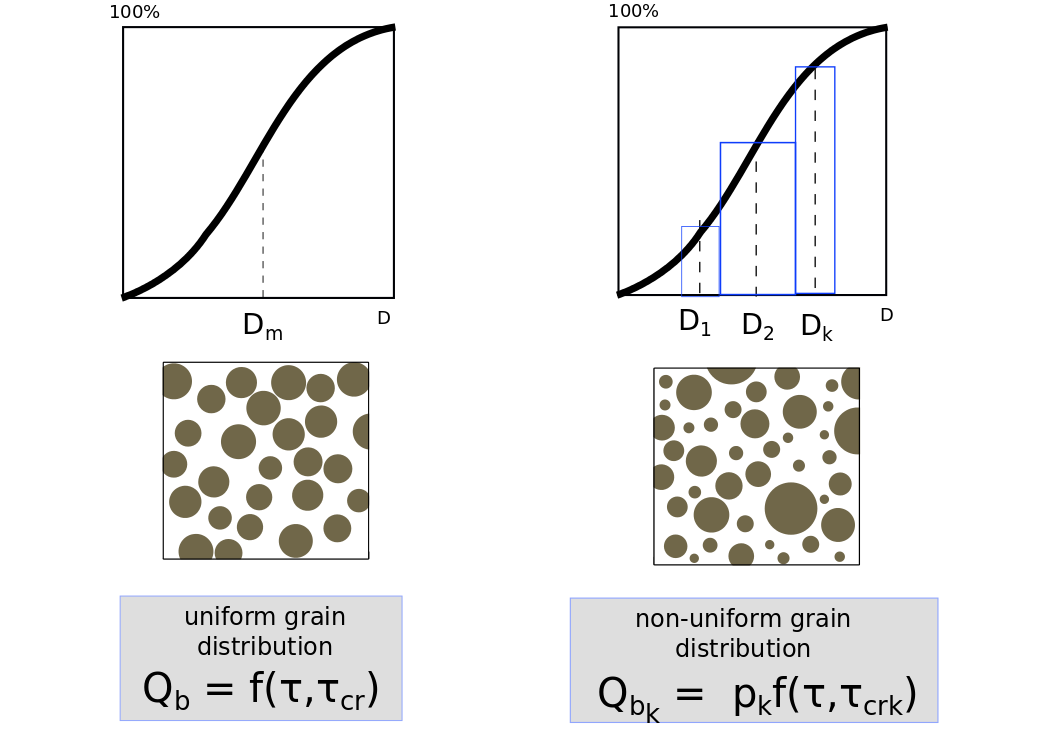
\includegraphics[scale=0.3]{./graphics/graded.png}
\end{center}
\end{figure}

\noindent
In the following, it is assumed a non-uniform sediment mixture divided into $N$ size classes. For bedload sediment transport processes, the evolution of bed topography is governed by the continuity equation, written in Cartesian coordinates for each grain size fraction as:

\begin{equation}
(1-\lambda)\left(\frac{\partial z_b}{\partial t}\right)_k+\frac{\partial Q_{bxk}}{\partial x}+\frac{\partial Q_{byk}}{\partial y} = 0,
\end{equation}
 where $Q_{bxk}, Q_{byk}$ (m$^2/$s) are the components of transport rates of the $k^{th}$ size class of bedload; $(\partial z_b/\partial t)_k$ (m/s) is the rate of change in bed elevation due to size class $k$; and $\lambda$ is the bed porosity.

For suspended sediment transport processes, the advection-diffusion equation is applied to determine the transport of each size class of suspended load:
\begin{multline}
\frac{\partial}{\partial t}\left(hC_k\right)+\frac{\partial (hUC_k)}{\partial x} + \frac{\partial (hVC_k)}{\partial y} \\
=\frac{\partial}{\partial x}\left[h\left(\varepsilon_s\frac{\partial C_k}{\partial x}\right)\right]+
\frac{\partial}{\partial y}\left[h\left(\varepsilon_s\frac{\partial C_k}{\partial y}\right)\right]+
\omega_{sk}\left(C_{eq_k}-C_{z_{ref}k}\right),
\end{multline}
where the subscript $k$ indicates the sediment size class index; $C_{z_{ref}k}$ and $C_{eq_k}$ are the actual and near-bed equilibrium concentrations of the $k^{th}$ size class of suspended load, respectively; and $\omega_{sk}$ (m/s) is the settling velocity of the $k^{th}$ size class.
\noindent
Bed changes due to suspended load transport for each grain size are:
\begin{equation}
(1-\lambda)\left(\frac{\partial z_b}{\partial t}\right)_k = \omega_{sk}\left(C_{z_{ref}k}-C_{eq_k}\right).
\end{equation}
\noindent
For either bedload or suspended sediment transport, the total rate in bed elevation change is then determined by:
\begin{equation}
\frac{\partial z_b}{\partial t} = \sum_{k=1}^N\left(\frac{\partial z_b}{\partial t}\right)_k.
\end{equation}
\noindent

The composition of the bed material may strongly vary along the vertical direction. The bed material above the nonerodible layer is often divided into multiple layers. In \sisyphe{}, the transport of non-uniform sediment particles can be computed using the \emph{active layer concept}~\cite{ElKadiAbderrezzak201675}. The uppermost bed layer is subdivided into two layers: an \textit{active or mixing layer}~\cite{Hirano1971} in contact with the flow, and a \textit{substrate layer} located directly below. The active layer supplies material that can be transported as bedload or suspended load and receives the deposited sediment material. At each loop on \sisyphe{}, the substratum exchanges material with the active layer in order to keep the active layer at a given thickness.

The active layer thickness depends on the flow and sediment characteristics~\cite{vanRijn87}. In \sisyphe{}, the active layer thickness is set by default to $3\times d_{50}$, being $d_{50}$ the median diameter of sediment material contained in the active layer.

%\begin{figure}[H]%
%\begin{center}
%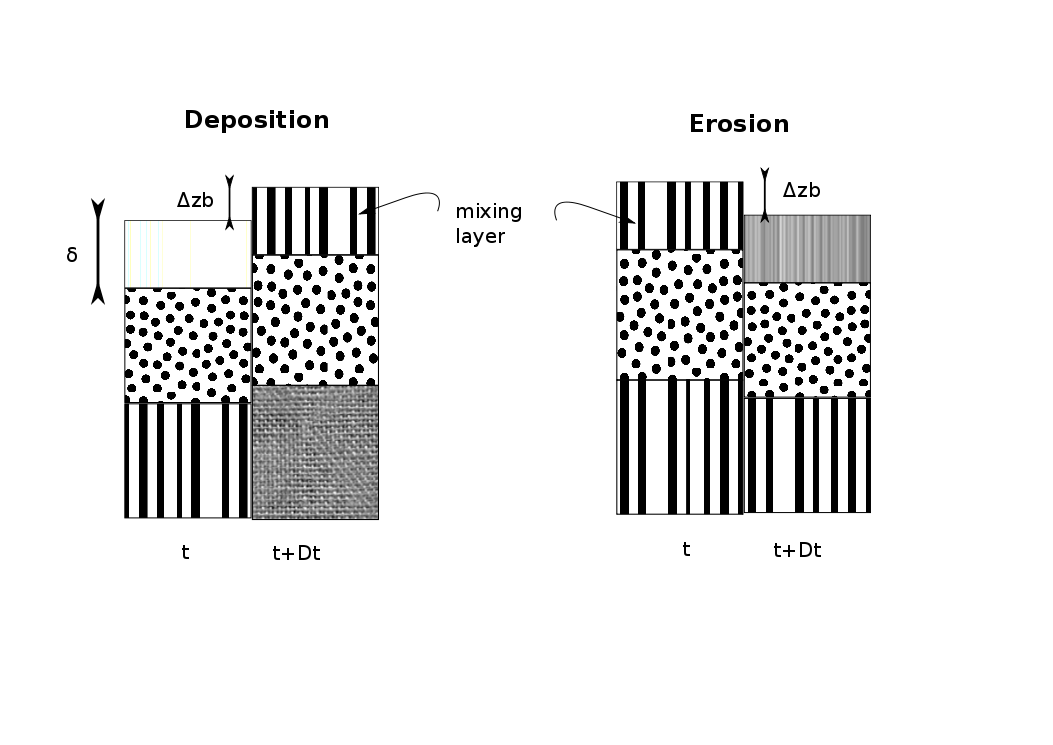
\includegraphics[scale=0.4]{./graphics/sorting.png}
%\end{center}
%\end{figure}

%-------------------------------------------------------------------------------
\section{Steering file setup for non-uniform sediment distribution}
%-------------------------------------------------------------------------------
Bedload and suspended load processes are set in the steering file with the keywords 
{\ttfamily BED LOAD} ({\ttfamily = YES} by default) and {\ttfamily SUSPENSION} ({\ttfamily = NO} by default), respectively.

Non-uniform sediment distribution can be set with the keyword {\ttfamily NUMBER OF SIZE-CLASSES OF BED MATERIAL} (integer type variable, set to {\ttfamily = 1} by default and limited to {\ttfamily = 20}).  Since the granulometry distribution is discretized in a number of classes, each sediment class is defined by its:
\begin{itemize}
\item Mean diameter {\ttfamily SEDIMENT DIAMETERS} (real type list, set to {\ttfamily = 0.01} m by default)
\item Initial volume fraction in the mixture {\ttfamily INITIAL FRACTION FOR PARTICULAR SIZE CLASS} (real type list, set to {\ttfamily = 1.,0.,0.,...} by default). The sum of the percentage of each class of material must always be equal to $1$.

\end{itemize}

%-------------------------------------------------------------------------------
\section{Non-uniform sediment distribution for bedload transport}
%-------------------------------------------------------------------------------
In \sisyphe{}, a constant active layer is set with the keyword {\ttfamily CONSTANT ACTIVE LAYER THICKNESS} (logical variable, set to {\ttfamily = YES} by default). The active layer thickness can be provided with the keyword {\ttfamily ACTIVE LAYER THICKNESS} (real variable, set to {\ttfamily = 100} m by default). %CHECK !!!

%-------------------------------------------------------------------------------
\subsection{Sediment transport formulas for non-uniform sediment distribution}
%-------------------------------------------------------------------------------
The choice of the transport formula is done with the keyword: {\ttfamily BED-LOAD TRANSPORT FORMULA} (integer type variable, set to {\ttfamily = 1} by default). Available formulas in \sisyphe{} are:
\begin{lstlisting}[frame=trBL]   
1 : MEYER-PETER & MULLER
2 : EINSTEIN-BROWN 
3 : ENGELUND-HANSEN + CHOLLET AND CUNGE 
30: ENGELUND-HANSEN 
6 : HUNZIKER 
7 : VAN RIJN
\end{lstlisting}
For each class, the Shields critical parameter can be either specified in the cas file or computed by \sisyphe{}: if the keyword {\ttfamily SHIELDS PARAMETERS} is not included in the steering file, \sisyphe{} computes this parameter for each class as a function of the grain size (fortran file \texttt{init\_sediment.f}).

%-------------------------------------------------------------------------------
\subsection{Hiding-exposure effects}
%-------------------------------------------------------------------------------
According to Einstein~\cite{Einstein}, in a sediment mix the finer grains are hidden behind and between the coarser grains and become less mobile than in a uniform sediment distribution. The coarser grains in a mixture are more exposed to the flow, ``feeling'' a larger drag force, and becoming more movable than in a uniform sediment distribution.

\begin{figure}[H]%
\begin{center}
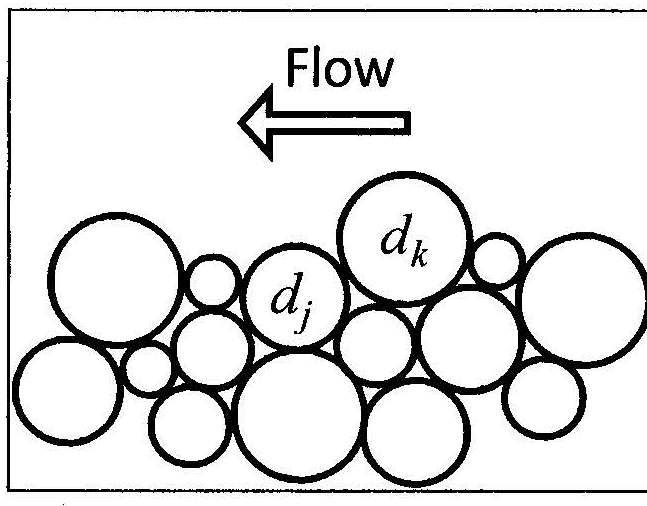
\includegraphics[scale=1.0]{./graphics/Fig_2_6_a.jpg}
\end{center}
\end{figure}

Prediction of sediment transport rates can be corrected with the \emph{hiding-exposure} factor. The Meyer-Peter \& M\"uller formula with \emph{hiding-exposure} correction factor $\zeta_i$ is:
\begin{equation}\label{eq:MPMhiding}
\Phi_{b_i}  = 8 p_i \left(\zeta_i \theta_i' -\theta_{cr} \right)^{3/2} 
\end{equation}
with $p_i$ the fraction of class $i$ in the active layer, $\theta_i'$ the Shields parameter (corrected by skin friction), $\theta_{cr}$ the critical Shields parameter.

In \sisyphe{}, the keyword {\ttfamily HIDING FACTOR FOR PARTICULAR SIZE CLASS} (real type list, set to {\ttfamily = 1., 1.,...} by default) sets the value of hiding factor for a particular size class and the keyword {\ttfamily HIDING FACTOR FORMULA} (integer type, set to {\ttfamily = 0} by default) allows the user to choose among different formulations. 

The Egiazaroff~\cite{Egiazaroff} and Ashida \& Michiue~\cite{Ashida} formulations modify the critical Shields parameter. The Karim and Kennedy~\cite{Karim} formula modifies the bedload transport rate
\begin{itemize}
\item \texttt{= 0}: ask for keyword {\ttfamily HIDING FACTOR FOR PARTICULAR SIZE CLASS}
\item \texttt{= 1}: formulation of Egiazaroff 
  \begin{equation*}
 \theta_{cr} = 0.047\zeta_i,\quad\text{with}\,\, \zeta_i = \left[\frac{\log (19)}{\log (19 D_i /D_m)} \right]^2 ,
\end{equation*}
with $D_i$ the grain size of class $i$ and $D_m$ the mean grain size of the surface layer.
\item \texttt{= 2}: formulation of Ashida \& Michiue, see~\cite{Ashida}

\item \texttt{= 4}: formulation of Karim and Kennedy, see~\cite{Karim}

\end{itemize}

The Hunziker's formula is an adaptation of the Meyer-Peter \& M\"{u}ller formula for fractional transport~\cite{Hunziker}. The volumetric sediment transport per sediment class is given by:
\begin{equation}\label{eq:Hunziker}
\Phi_{b_i}  = 5 p_i \left[\zeta_i\left( \theta_i' -\theta_{cm} \right) \right]^{3/2} \quad\text{if}\quad \theta_i' > \theta_{cm}, 
\end{equation}
with $p_i$ the fraction of class $i$ in the active layer, $\theta_i'$ the Shields parameter (corrected by skin friction), 
$\theta_{cm} = \theta_{cr}\left(D_{mo}/D_m\right)^{0.33}$ the corrected critical Shields parameter, $\theta_{cr}$ the critical Shields parameter, $\zeta_{i} =\left(D_i/D_m\right)^{-\alpha_{hu}}$ the hiding factor, $\alpha_{hu}$ a coefficient, $D_i$ the grain size of class $i$, $D_m$ the mean grain size of the surface layer, $D_{mo}$ the mean grain size of the under layer.

According to Hunziker, stability problems may occur outside the parameter range $\alpha \leq 2.3$ and $D_i/D_m \geq 0.25$.


%-------------------------------------------------------------------------------
\section{Non-uniform sediment distribution for suspended sediment transport}
%-------------------------------------------------------------------------------
For this case, set {\ttfamily BED LOAD = NO} and {\ttfamily SUSPENSION = YES}.

The initial condition value of the concentration for each class can be specified through the keyword {\ttfamily INITIAL SUSPENSION CONCENTRATIONS} (real type list, {\ttfamily = 0.0, 0.0, 0.0,...} by default). Boundary conditions for sediment concentration can be:
\begin{itemize}
\item Specified by \textbf{depth-averaged volume concentration values} at a boundary for each class through the keyword {\ttfamily CONCENTRATION PER CLASS AT BOUNDARIES} (real type list, see example below) $\rightarrow$ boundary 1 (class 1, class2, etc.), then boundary 2, (class 1, class2, etc.), then...
\item Computed for each class through the keyword {\ttfamily EQUILIBRIUM INFLOW CONCENTRATION} (logical type variable, {\ttfamily = NO} by default) and according to the choice of the formula of equilibrium near-bed concentration ({\ttfamily REFERENCE CONCENTRATION FORMULA = 1} by default) 
\item Fortran file: \texttt{conlit.f}
\end{itemize}

Keywords used for uniform sediment distribution are also valid for non-uniform distribution: {\ttfamily SKIN FRICTION CORRECTION}, {\ttfamily RATIO BETWEEN SKIN FRICTION AND MEAN DIAMETER}, {\ttfamily MASS CONCENTRATION}, etc.

For each class, the settling velocity can be either specified in the cas file or computed by \sisyphe{}:
\begin{itemize}
\item If the keyword {\ttfamily SETTLING VELOCITIES} is not included in the steering file, \sisyphe{} computes the settling velocity for each sediment class by the Stokes, Zanke or van Rijn formulae depending on the grain size (fortran file \texttt{vitchu\_sisyphe.f})
\end{itemize}

\section{Bed structure: discretization by layers}
The number of layers is specified with the keyword {\ttfamily NUMBER OF BED LOAD MODEL LAYERS} (real type list, set to {\ttfamily = 2} by default), variable \texttt{NOMBLAY}
\begin{itemize}
\item If {\ttfamily = 2}: the initial volume fraction provided in the steering file
\item If {\ttfamily > 2}: the initial volume fraction and layer thickness must be provided with the Fortran subroutine \texttt{init\_compo.f}
\end{itemize}

\begin{figure}[H]%
\begin{center}
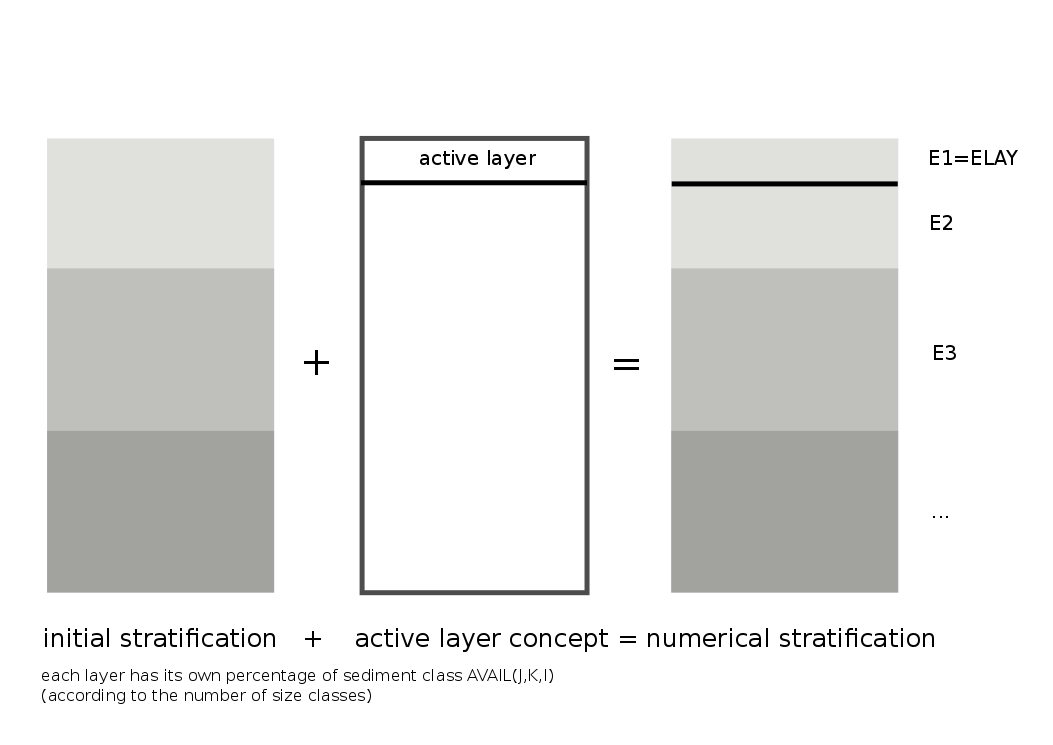
\includegraphics[scale=0.4]{./graphics/layers_1.png}
\end{center}
\end{figure}

In the subroutine \texttt{init\_compo.f} we define for size class \texttt{I}, each node \texttt{J} and each layer \texttt{K}:
\begin{itemize}
\item the thickness \texttt{ES(J,K)}
\item the initial volume fraction \texttt{AVAIL(J,K,I)}
\end{itemize}

\pagebreak

Example for 3 sediment classes and 3 layers:
\begin{lstlisting}[frame=trBL]   
    DO J=1,NPOIN
        NCOUCHES(J) = 3
        AVAIL(J,1,1) = AVA0(1) 
        AVAIL(J,1,2) = AVA0(2) 
        AVAIL(J,1,3) = AVA0(3) 
        AVAIL(J,2,1) = 0.
        AVAIL(J,2,2) = 0.5
        AVAIL(J,2,3) = 0.5
        AVAIL(J,3,1) = 0.90
        AVAIL(J,3,2) = 0.
        AVAIL(J,3,3) = 0.10 
        ES(J,1) = 10.D0
        ES(J,2) = 30.D0
    ENDDO
\end{lstlisting}
Above, \texttt{AVA0} is the list with the initial fractions provided with {\ttfamily INITIAL FRACTION FOR PARTICULAR SIZE CLASS}.

\begin{WarningBlock}{Note:}
In the \sisyphe steering file, the keywords \telkey{COMPUTATION CONTINUED = YES} and \telkey{PREVIOUS SEDIMENTOLOGICAL COMPUTATION FILE = [name file]} must be provided
to ensure that the information contained in the layers from the previous computation are accounted in the current simulation.
\end{WarningBlock}
  


%-------------------------------------------------------------------------------
\subsection{Useful graphical printouts}
%-------------------------------------------------------------------------------
\subsubsection{Bedload}
The keyword {\ttfamily VARIABLES FOR GRAPHIC PRINTOUTS} allows the use of useful printouts for non-uniform sediments:
\begin{lstlisting}[frame=trBL]   
E="bottom evolution (m)";
M="bed-load discharge (m2/s)";
1Ai="fraction of sediment of class i 
in the first layer";
2Ai="fraction of sediment of class i 
in the second layer";
kAi="fraction of sediment of class i 
in the k layer";
kES="thickness of the k layer";
QSi="bed load transport rate of sediment 
of class i"
\end{lstlisting}
Above, \texttt{*kES} means print the thickness of all layers; \texttt{*A*} means print all fractions for all layers.

\subsubsection{Suspended-load}
The keyword {\ttfamily VARIABLES FOR GRAPHIC PRINTOUTS} allows the use of useful printouts for non-uniform sediments:
\begin{lstlisting}[frame=trBL]   
QSSUSP="suspended load transport rate (m2/s)";
CSi="concentration volumic or mass concentration 
for class i"
kCONC="concentration of bed layer k"
\end{lstlisting}
Above, \texttt{CS*} prints the concentration for all fractions.


%-------------------------------------------------------------------------------
\section{Continuous Vertical Grain Sorting Model}
%-------------------------------------------------------------------------------
Sediment sorting of sediments using the continuous vertical model are implemented in \sisyphe{} according to~\cite{Merkeletal2012}. Further details on suitable applications of this model are presented in~\cite{Merkel2017}.
